\section{滤波器}

这一章主要讨论滤波器的设计和实现。滤波器是信号处理中的一个重要部分,
它可以用来去除噪声,提取信号,以及对信号进行分析。滤波器的设计是一个复杂的过程,
需要根据具体的应用来选择合适的滤波器类型和参数。
在本章中,我们将讨论滤波器的基本原理,以及如何设计和实现滤波器。

\begin{note}
    此小节还未完成。
\end{note}

\subsection{滤波器的表示}

\subsubsection{滤波器的表示}

\begin{definition}
    \bd{滤波器}是以特定方式改变信号的频率特性,从而变换信号的处理系统。
    滤波器一般有如下类别,如图 \ref{fig:filter-types} 所示:
    \begin{enumerate}[label=(\arabic*)]
        \item 高通滤波器(HP)
        \item 低通滤波器(LP)
        \item 带通滤波器(BP)
        \item 带阻滤波器(BS)
        \item 全通滤波器(AP)
    \end{enumerate}
    \begin{figure}[H]
        \centering
        \includegraphics[width=0.8\textwidth]{chap4/img/filter_types.png}
        \caption{滤波器类型}
        \label{fig:filter-types}
    \end{figure}

    滤波器也可以被分为\bd{模拟滤波器}和\bd{数字滤波器}。
    \begin{itemize}
        \item \bd{模拟滤波器}是由电阻、电容、电感等部件构成的电路。
            滤波器特性对所用部件的物理标称值非常敏感,而且,
            有些部件的物理特性会随温度变化而改变。
        \item \bd{数字滤波器}是用软件实现的,很少依赖硬件。滤波软件
            只是一系列程序指令。虽然它是在硬件平台上运行,但
            是硬件平台本身并不决定滤波器的性能。数字滤波器的
            性能是由\bd{一组系数}确定的。
    \end{itemize}
    数字滤波器的实现方式一般有以下几种:
    \begin{enumerate}
        \item 用流图计算滤波器的输出。
        \item 用差分方程计算滤波器的输出。
        \item 用卷积过程计算滤波器的输出。
        \item 用 DTFT 直接改变信号频谱。
    \end{enumerate}
\end{definition}

\begin{example}[(低通)滤波器的滤波特性参数]
    \begin{figure}[H]
        \centering
        % TODO: 需要重新截图
        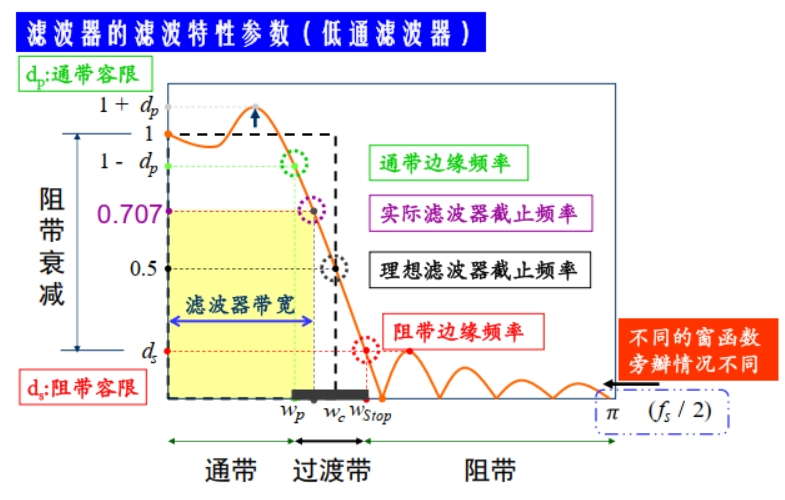
\includegraphics[width=0.8\textwidth]{chap4/img/filter_characteristics.png}
        \caption{滤波器的滤波特性参数}
        \label{fig:filter-characteristics}
    \end{figure}
    虚线表示的是\bd{理想低通滤波器}的滤波特性,实线表示的是\bd{窗函数法}设计
    得到的\bd{实际低通滤波器}的滤波特性。
\end{example}

\subsubsection{什么是系统}

滤波器是以特定方式改变信号的频率特性的系统。那么,什么是系统呢?

\begin{definition}[系统]
    \bd{系统}是由若干相互作用和相互依赖的事物组合而成的具有特定功能的整体。例如,
    计算机系统、医疗系统、雷达导航系统等。

    通俗地说,对信号处理的各种环境都可以被称为系统。在信号处理领域,系统是为了
    传送信号或对信号进行加工处理而构成的某种组合。这种组合,既可以有对应的物理设备,
    如电容、放大器等,也可以是纯粹的算法,如计算机软件程序等;关键在于,系统是
    一个具有``特定功能的整体''。
\end{definition}

\begin{example}[系统的分类]
    
\end{example}

\begin{example}[常见的系统类型]
    这里仅讨论线性、
\end{example}

\begin{remark}
    为什么要研究滤波器这一系统呢?
    因为我们需要对信号进行处理,而滤波器是信号处理的重要工具。
    \begin{itemize}
        \item 对于具有特定参数的系统,它具有何种处理信号的特性?
            \subitem 即:分析信号在通过系统后,信号的特性会发生怎样的变化?
            % \end{itemize}
        \item 对于给定的传输和处理信号的要求,如何设计并实现一个与其相匹配的系统?
            \begin{itemize}
                \item 即:如何设计并实现系统,使系统满足信号处理的要求?系统应具有怎样的功能和参数?
            \end{itemize}
    \end{itemize}
\end{remark}
\begin{example}[系统的描述方法]
    
\end{example}

\subsubsection{系统响应的分类}

\begin{example}[]
    常见的两种系统响应是\bd{零输入响应}和\bd{零状态响应}。
    \begin{itemize}
        \item 
    \end{itemize}

\end{example}

\subsubsection{FIR 和 IIR 滤波器}

\begin{example}
    \label{exercise:serial-flow-chart}
    写出如图 \ref{fig:serial-flow-chart} 所示级联流图的差分方程。
    \begin{figure}[H]
        \centering
        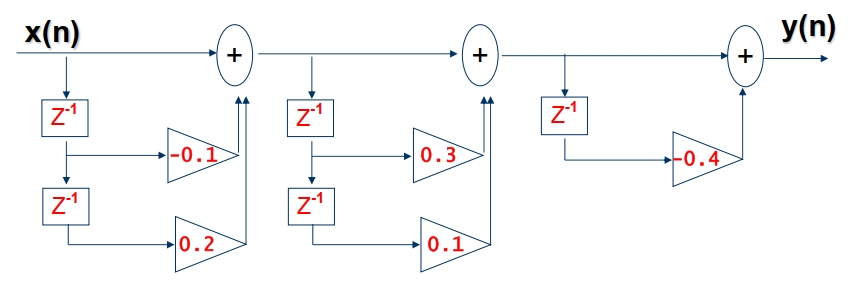
\includegraphics[width=0.8\textwidth]{chap4/img/serial_flow_chart.png}
        \caption{例 \theexample~ 的级联流图}
        \label{fig:serial-flow-chart}
    \end{figure}
\end{example}

\begin{solution}
    不妨设 $x(n) = x_1(n), y(n) = y_3(n)$,
    以及 $y_1(n) = x_2(n), y_2(n) = x_3(n)$,则如图 \ref{fig:serial-flow-chart-annotated} 所示,
    \begin{align*}
        y_1(n) & = x_1(n) - 0.1x_1(n - 1) + 0.2x_1(n - 2), \\
        y_2(n) & = x_2(n) + 0.3x_2(n - 1) + 0.1x_2(n - 2), \\
        y_3(n) & = x_3(n) - 0.4x_3(n - 1).
    \end{align*}
    \begin{figure}[H]
        \centering
        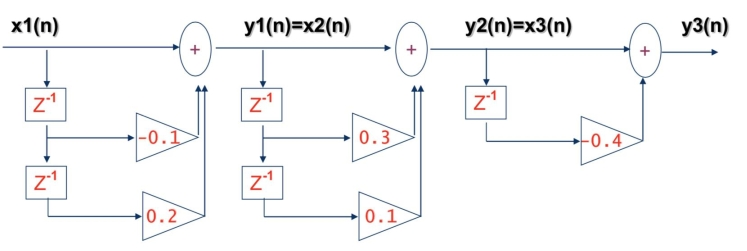
\includegraphics[width=0.8\textwidth]{chap4/img/serial_flow_chart_annotated.png}
        \caption{例 \theexample~ 的级联流图(带标注)}
        \label{fig:serial-flow-chart-annotated}
    \end{figure}
    将 $y_1(n)$ 代入 $y_2(n)$ 的表达式中,将 $y_2(n)$ 代入 $y_3(n)$ 的表达式中,
    可得级联流图的差分方程为
    \begin{align*}
        y_3(n) = x_1(n) - 0.2x_1(n - 1) + 0.19x_1(n - 2) - 0.058x_1(n - 3) - 0.008x_1(n - 5).
    \end{align*}
\end{solution}

% TODO: 4.1 第一个 PPT

\subsubsection{用差分方程表示系统}

\subsubsection{用流图表示系统}

\subsubsection{用脉冲响应表示系统}

\begin{theorem}
    设某滤波器的脉冲响应为 $h(n)$,某输入信号为 $x(n)$。则输入信号可以表示
    为一系列脉冲函数之和:
    \begin{align*}
        x(n) = \sum_{k = -\infty}^{+\infty}x(k)\delta(n - k).
    \end{align*}
    当输入单位脉冲时,即 $x(n) = \delta(n)$,滤波器的输出响应为 $h(n)$,
    则根据 LTI 系统的线性性质和时不变性特性,输入 $x(n)$ 时的输出为
    \begin{align*}
        y(n) = \sum_{k = -\infty}^{+\infty}x(k)h(n - k) = x(n) * h(n).
    \end{align*}
    
    即,\bd{数字滤波器的输出等于输入信号,与脉冲响应的卷积}。
\end{theorem}

\begin{property}[差分方程与卷积运算]
    \label{property:diff-equation-convolution}
    写出 FIR 和 IIR 系统的差分方程如下:
    \begin{align*}
        \sum_{k = 0}^{N}b(k)y(n - k) & = \sum_{k = 0}^{M}a(k)x(n - k) & \text{(IIR)} \\
        y(n) & = \sum_{k = 0}^{M}a(k)x(n - k) & \text{(FIR)}
    \end{align*}
    在 FIR 系统的差分方程中,实际上系数 $a(k)$ 就是系统的脉冲响应 $h(k)$。也就是说,有
    \begin{align*}
        y(n) = a(n) * x(n) \qquad \text{(FIR)}
    \end{align*}

    卷积和差分方程都可以用来计算滤波器的输出。对于 FIR 而言,卷积运算和差分方程都适用;
    对于 IIR 而言,差分方程更加方便。
\end{property}

\begin{remark}
    由以上讨论可知,描述系统的方式有以下几种:
    \begin{itemize}
        \item 系统的差分方程
        \item 流图
        \item 数字系统的脉冲响应 $h(n)$
    \end{itemize}
\end{remark}

\begin{exercise}
    \label{exercise:LTI-stable}
    证明:某 LTI 系统稳定的充要条件是
    \begin{align*}
        \sum_{n = -\infty}^{\infty} \abs{h(n)} = P < \infty.
    \end{align*}
    其中 $h(n)$ 为系统的单位脉冲响应,$P$ 为一个常数。
\end{exercise}

\begin{proof}
    首先证明必要性。不妨设 $\sum_{n= -\infty}^{+\infty}\abs{h(n)} = A$,
    对任意的有界输入 $x(n)$,设 $\forall n, \abs{x(n)} < B$。则
    \begin{align*}
        \abs{y(n)} & = \abs{x(n) * h(n)} = \abs{\sum_{k = -\infty}^{+\infty}h(k)x(n - k)} \\
        & \le \sum_{k = -\infty}^{+\infty} \abs{h(k)} \cdot \abs{x(n - k)} \\
        & < B \sum_{k = -\infty}^{+\infty} \abs{h(k)} = AB
    \end{align*}
    也有界。

    接下来证明充分性。使用反证法,设 $\sum_{n = -\infty}^{\infty} \abs{h(n)}$ 发散时,系统稳定。
    考虑输入
    \begin{align*}
        x(n) = \begin{cases}
                0, & h(-n) = 0, \\
                \sgn{h(-n)}, & h(-n) \neq 0.
            \end{cases}
    \end{align*}
    显然输入是有界的,且 $\forall n, \abs{x(n)} \le 1$。而
    \begin{align*}
        y(0) & = (x * h)(0) = \sum_{k = -\infty}^{+\infty}h(k)x(-k) \\
        & = \sum_{k = -\infty}^{+\infty}h(k) \cdot \sgn{h(k)} \\
        & = \sum_{k = -\infty}^{+\infty}\abs{h(k)}
    \end{align*}
    这个结果发散,说明输出是无界的,这与系统稳定相矛盾。故假设不成立,
    也就是说 $\sum_{n = -\infty}^{\infty} \abs{h(n)}$ 是收敛的。

    命题得证。
\end{proof}

\begin{property}[系统的串、并联组合]
    \label{property:parallel-serial-system}
    系统在串联和并联的情况下,其传递函数的组合规律如下:
    \begin{itemize}
        \item 两个系统的\bd{并联}后新系统的单位冲激响应是并联子系统的单位冲激响应之和,
            传递函数是并联子系统的传递函数之和。如图 \ref{fig:parallel-system} 所示,
            是一个并联系统。
            \begin{align*}
                h(n) = h_1(n) + h_2(n), \quad H(z) = H_1(z) + H_2(z).
            \end{align*}
        \item 两个系统的\bd{串联}后新系统的单位冲激响应是串联子系统的单位冲激响应的卷积,
            传递函数是串联子系统的传递函数的乘积。如图 \ref{fig:serial-system} 所示,
            是一个串联系统。
            \begin{align*}
                h(n) = h_1(n) * h_2(n), \quad H(z) = H_1(z) \cdot H_2(z).
            \end{align*}
    \end{itemize}
    \begin{figure}[H]
        \centering
        \begin{subfigure}{0.45\textwidth}
            \centering
            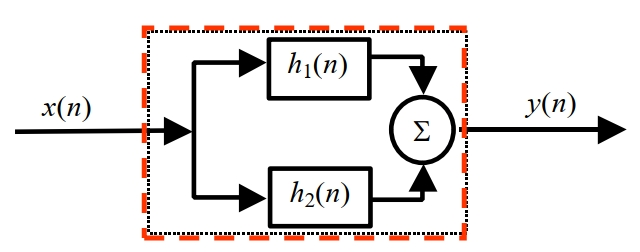
\includegraphics[width=\textwidth]{chap4/img/parallel_system.png}
            \caption{并联系统}
            \label{fig:parallel-system}
        \end{subfigure}
        \begin{subfigure}{0.45\textwidth}
            \centering
            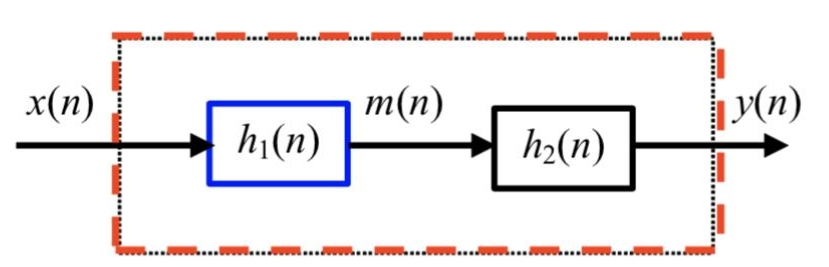
\includegraphics[width=\textwidth]{chap4/img/serial_system.png}
            \caption{串联系统}
            \label{fig:serial-system}
        \end{subfigure}
        \caption{系统的串、并联组合}
    \end{figure}
\end{property}

\subsubsection{系统的频率响应}

\begin{definition}[系统的频率响应]
    \bd{系统的频率响应},简称\bd{频响},反映了系统对激励中各频率分量的幅度和相位的影响。
    通常为复值函数,写成
    \begin{align*}
        H(\omega) = \abs{H(\omega)}\mathe^{\mathi \varphi(\omega)}.
    \end{align*}
    其中,$\abs{H(\omega)}$ 是\bd{幅频响应},$\varphi(\omega)$ 是\bd{相频响应}。
    
    接下来,我们将从 DTFT 的角度来理解频率响应函数和差分方程之间的关系。
    \begin{align*}
        H(\omega) = \sum_{n = -\infty}^{+\infty}h(n)\mathe^{\mathi n \omega}.
    \end{align*}
    由上式可以看出,$H(\omega)$ 是周期函数,分别关于 $\omega = 0$ 和 $\omega = \omega_s/2$ 共轭对称。
\end{definition}

\begin{example}[FIR 系统的频率响应]
    设有 FIR 系统,其差分方程为
    \begin{align*}
        y(n) = \sum_{k = -\infty}^{+\infty}x(k)h(n - k),
    \end{align*}
    即 $y(n) = x(n) * h(n)$。对等式左右求 DTFT,得
    \begin{align*}
        Y(\omega) = X(\omega) H(\omega).
    \end{align*}
    因此,滤波器的\bd{频率响应}为
    \begin{align*}
        H(\omega) = Y(\omega) / X(\omega) = \DTFT{h(n)}.
    \end{align*}
\end{example}

\begin{theorem}[频率响应与差分方程]
    \label{thm:freq-response-diff-equation}
    设有差分方程
    \begin{align*}
        \sum_{k = 0}^{N}b(k)y(n - k) = \sum_{k = 0}^{M}a(k)x(n - k),
    \end{align*}
    其中 $x(n), y(n)$ 的 DTFT 分别为 $X(\omega), Y(\omega)$,则系统的频率响应为
    \begin{align*}
        H(\omega) = \frac{Y(\omega)}{X(\omega)} = \frac{\sum_{k = 0}^{M}a(k)\mathe^{-\mathi k \omega}}{\sum_{k = 0}^{N}b(k)\mathe^{-\mathi k \omega}}.
    \end{align*}
\end{theorem}

\begin{proof}
    考虑差分方程
    \begin{align*}
        \sum_{k = 0}^{N}b(k)y(n - k) = \sum_{k = 0}^{M}a(k)x(n - k),
    \end{align*}
    即 $b(n) * y(n) = a(n) * x(n)$。对等式左右求 DTFT,得
    \begin{align*}
        Y(\omega) \sum_{k = 0}^{N}b(k)\mathe^{-\mathi k\omega} = X(\omega)\sum_{k = 0}^{M}a(k)\mathe^{-\mathi k\omega}.
    \end{align*}
    此即
    \begin{align*}
        H(\omega) = \frac{Y(\omega)}{X(\omega)} = \frac{\sum_{k = 0}^{M}a(k)\mathe^{-\mathi k \omega}}{\sum_{k = 0}^{N}b(k)\mathe^{-\mathi k \omega}}.
    \end{align*}
    命题得证。
\end{proof}

\begin{remark}
    对于定理 \ref{thm:freq-response-diff-equation},我们可以进一步讨论。
    对于差分方程
    \begin{align*}
        \sum_{k = 0}^{N}b(k)y(n - k) = \sum_{k = 0}^{M}a(k)x(n - k),
    \end{align*}
    \begin{itemize}
        \item 输出信号可以由输入信号的当前(及过去)与输出信号的过去的线性组合表示。
        \item 输出信号与其延迟信号的叠加,等于输入信号与其延迟信号的叠加。
    \end{itemize}
    它们的 DTFT 相等,说明\bd{原信号在时域叠加,结果信号的频谱也是原信号频谱的叠加}。
\end{remark}

\begin{exercise}
    已知某因果系统的流图如 \ref{fig:chap4-part1-quiz2} 所示,且满足 $0 < a < 1$.
    求系统的差分方程、系统的频率响应、以及系统的幅频响应图,
    并说明系统相当于何种滤波器(高通、低通、带通、带阻、全通)。
    \begin{figure}[H]
        \centering
        \tikzstyle{block} = [draw, rectangle, minimum height=1cm, minimum width=1cm]
        \tikzstyle{circ} = [draw, fill, circle, inner sep=1.5pt]
        \tikzstyle{no-circ} = [draw, circle, inner sep=0pt]
        \tikzstyle{sum} = [draw, circle]
        \tikzstyle{line} = [draw, -latex]
        \tikzstyle{no-arrow-line} = [draw, -]
        \tikzstyle{gainx} = [draw, isosceles triangle, isosceles triangle apex angle=60]
        \tikzstyle{gainy} = [draw, isosceles triangle, isosceles triangle apex angle=60, shape border rotate=180]
        \begin{tikzpicture}
            \node [name=input] (input) {$x(n)$};
    
    
            \node [sum, right of=input, xshift=4cm] (sum) {$+$};
            \node [circ, right of=sum, xshift=4cm] (circy) {};
            \path [no-arrow-line] (sum) -- (circy);
            \node [name=output, right of=circy, xshift=1cm] (output) {$y(n)$};
            \path [line] (circy) -- (output);
    
    
            \node [block, below of=circy, yshift=-1cm] (zy1) {$Z^{-1}$};
            \path [line] (circy) -- (zy1);
    
            \path [line] (input) -- (sum);
            \node [gainy, below of=zy1, xshift=-2cm, yshift=-0.5cm] (zgy1) {$a$};
            \path [line] (zy1) |- (zgy1);
            \path [line] (zgy1.west) -- (sum);
        \end{tikzpicture}
        \caption{习题 \theexercise~ 的信号流图}
        \label{fig:chap4-part1-quiz2}
    \end{figure}
\end{exercise}

\begin{solution}
    由图可知系统的差分方程为
    \begin{align*}
        y(n) = ay(n - 1) + x(n).
    \end{align*}
    因此,系统的频率响应为
    \begin{align*}
        H(\omega) = \frac{\mathe^{\mathi \omega}}{\mathe^{\mathi \omega} - a}
            = \frac{1}{(1 - a\cos\omega) + \mathi a\sin\omega}
    \end{align*}
    所以其幅频响应函数为
    \begin{align*}
        \abs{H(\omega)} & = \frac{1}{\sqrt{(1 - a\cos\omega)^2 + a^2\sin^2\omega}} \\
        & = \frac{1}{\sqrt{1 + a^2 - 2a\cos\omega}}
    \end{align*}
    如图 \ref{fig:chap4-part1-quiz2-plot} 所示,其幅频响应函数为一个低通滤波器。
    \begin{figure}[H]
        \centering
        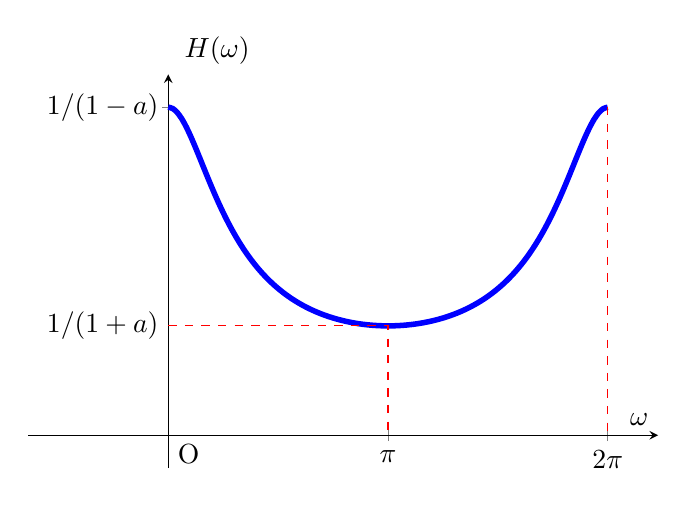
\begin{tikzpicture}
            \begin{axis}[
                axis lines = middle,
                xlabel = {$\omega$},
                ylabel = {$\abs{H(\omega)}$},
                ylabel style={at={(rel axis cs:0.3, 1)}, anchor=south},
                xmin = -2, xmax = 7,
                ymin = -0.2, ymax = 2.2,
                xtick = {0, 3.14, 6.28},
                xticklabels = {$0$, $\pi$, $2\pi$},
                ytick = {0, 2},
                yticklabels = {$ $, $ $},
                scale only axis,
                width = 8cm,
                height = 5cm,
            ]
            \addplot[domain=0:6.28, samples=100, smooth, line width=2pt, blue] {1 / sqrt(1.25 - cos(deg(x)))};
            \addplot[dashed, red] coordinates {(0, 0.667) (3.14, 0.667) (3.14, 0)};
            \addplot[dashed, red] coordinates {(6.28, 2) (6.28, 0)};
            \node at (axis cs:0, 0) [anchor=north west] {O};
            \node at (axis cs:0, 0.667) [anchor=east] {$1/(1 + a)$};
            \node at (axis cs:0, 2) [anchor=east] {$1/(1 - a)$};
            \end{axis}
        \end{tikzpicture}
        \caption{习题 \theexercise~ 的幅频响应函数}
        \label{fig:chap4-part1-quiz2-plot}
    \end{figure}
\end{solution}

\subsubsection{由差分方程求脉冲响应函数}

在性质 \ref{property:diff-equation-convolution} 中我们已经知道,
对于 FIR 系统,$h(n) = a(n)$。那么对于 IIR 系统,
\begin{align*}
    \sum_{k = 0}^{N}b(k)y(n - k) = \sum_{k = 0}^{M}a(k)x(n - k).
\end{align*}
我们应该如何求解 $h(n)$ 呢?可以考虑使用更强大的工具——Z 变换。

\subsection{Z 变换}

Z 变换是离散时间信号与系统的理论研究中的一种重要的数学工具。
它把离散的数学模型(差分方程)转换为简单的代数方程,
使其求解过程得以简化。

\subsubsection{Z 变换的定义}

\begin{definition}[Z 变换的定义]
    设 $x(n)$ 是一个离散时间信号,其\bd{单边 Z 变换}的定义为
    \begin{align*}
        X(z) = \sum_{n = 0}^{+\infty} x(n) z^{-n},
    \end{align*}
    \bd{双边 Z 变换}的定义为
    \begin{align*}
        X(z) = \sum_{n=-\infty}^{+\infty} x(n) z^{-n},
    \end{align*}
    记作 $X(z) = \mathcal{Z}[x(n)]$。
\end{definition}

\begin{remark}[Z 变换和 DTFT 之间的关系]
    回忆 DTFT 的定义,我们有
    \begin{align*}
        X(\omega) = \sum_{n=-\infty}^{+\infty} x(n) \mathe^{-\mathi\omega n},
    \end{align*}
    注意到 $\mathe^{-\mathi\omega n} = \left(\mathe^{\mathi\omega}\right)^{-n}$,
    因此,DTFT 也可以写为
    \begin{align*}
        X(\omega) = \sum_{n=-\infty}^{+\infty} x(n) \left(\mathe^{\mathi\omega}\right)^{-n},
    \end{align*}
    这具有类似于 Z 变换的形式。DTFT 的变换核是 $\mathe^{-\mathi\omega n}$,
    将其换成 $z^{-n}$,可以看做是变换核对应的取值从单位圆上的点($\mathe^{\mathi\omega}$)
    变成了整个复平面上的点($z$)。
\end{remark}

\subsubsection{Z 变换的收敛域}

\begin{definition}[Z 变换的收敛域]
    考虑 Z 变换
    \begin{align*}
        X(z) = \mathcal{Z}[x(n)] = \sum_{n=-\infty}^{+\infty} x(n) z^{-n},
    \end{align*}
    它具有幂级数求和的形式。显然当 $z$ 固定时,它不一定对所有的序列 $x(n)$ 都收敛;
    当序列 $x(n)$ 固定时,它不一定对所有的 $z$ 都收敛。

    但如果给定了序列 $x(n)$,则可以求出使得 $X(z)$ 收敛的 $z$ 的取值范围。
    我们称使 $X(z)$ 收敛的 $z$ 的取值范围为 $X(z)$ 的\bd{收敛域},简记为 ROC。
\end{definition}

\begin{property}[Z 变换的 ROC 的性质]
    Z 变换的 ROC 一般具有以下性质:
    \begin{enumerate}
        \item ROC 的一般形式是复平面上以原点为中心的圆环。
        \item ROC \bd{不包含极点},而且常以极点作为 ROC 的边界。
        \item 在 ROC 内,ZT 及其导数是 $z$ 的连续函数,即 ZT 是 ROC 内每一点的解析函数。
    \end{enumerate}
\end{property}

\begin{example}[Z 变换 ROC 的求解]
    Z 变换得到的序列是一个幂级数,幂级数的收敛域称为\bd{收敛圆},
    收敛圆的半径称为幂级数的\bd{收敛半径}。收敛半径的求法有两种:
    \begin{itemize}
        \item 利用比值判别法,
            \begin{align*}
                \lim_{n \to +\infty}\abs{\frac{a_{n+1}}{a_n}} = \rho.
            \end{align*}
        \item 利用根值判别法,
            \begin{align*}
                \lim_{n \to +\infty}\sqrt[n]{\abs{a_n}} = \rho.
            \end{align*}
    \end{itemize}
    收敛半径 $R$ 与 $\rho$ 的关系为:
    \begin{itemize}
        \item 若 $\rho = 0$,则 $R = +\infty$。
        \item 若 $\rho = +\infty$,则 $R = 0$。
        \item 对于其他情况,$R = 1/\rho$。
    \end{itemize}
\end{example}

\begin{property}[有限长序列的 ROC]
    \bd{有限长序列} $x(n)$ 在 $n < n_1$ 或 $n > n_2$ 时为 $0$,
    则其 Z 变换为
    \begin{align*}
        X(z) = \sum_{n=n_1}^{n_2} x(n) z^{-n},
    \end{align*}
    其中 $n_1 < n_2$。其 ROC \bd{至少}是 $0 < \abs{z} < +\infty$。

    序列的左右端点只会影响其在 $z = 0$ 和 $z = +\infty$ 处的收敛性:
    \begin{itemize}
        \item 若 $n_1 < 0 < n_2$,则 ROC 为 $0 < \abs{z} < +\infty$。
        \item 若 $n_1 < n_2 \le 0$,则 ROC 为 $0 \le \abs{z} < +\infty$。
        \item 若 $0 \le n_1 < n_2$,则 ROC 为 $0 < \abs{z} \le +\infty$。
    \end{itemize}
\end{property}

\begin{property}[右边序列的 ROC]
    \bd{右边序列} $x(n)$ 在 $n < n_1$ 时为 $0$,则其 Z 变换为
    \begin{align*}
        X(z) = \sum_{n=n_1}^{+\infty} x(n) z^{-n}.
    \end{align*}
    若满足
    \begin{align*}
        \lim_{n \to +\infty}\sqrt[n]{\abs{x(n)z^{-n}}} < 1,
    \end{align*}
    则右边序列的收敛域为
    \begin{align*}
        \abs{z} > \lim_{n \to +\infty}\sqrt[n]{\abs{x(n)}} = R_{x1}.
    \end{align*}
    因此,\bd{右边序列的 ROC 是半径为 $R_{x1}$ 的圆外部分}。

    序列的左右端点只会影响其在 $z = +\infty$ 处的收敛性:
    \begin{itemize}
        \item 若 $n_1 < 0$,则 ROC 为 $R_{x1} < \abs{z} < +\infty$。
        \item 若 $n_1 \ge 0$,则 ROC 为 $R_{x1} < \abs{z} \le +\infty$。
    \end{itemize}
\end{property}

\begin{property}[左边序列的 ROC]
    \bd{左边序列} $x(n)$ 在 $n > n_2$ 时为 $0$,则其 Z 变换为
    \begin{align*}
        X(z) = \sum_{n=-\infty}^{n_2} x(n) z^{-n}.
    \end{align*}
    若满足
    \begin{align*}
        \lim_{n \to +\infty}\sqrt[n]{\abs{x(-n)z^n}} < 1,
    \end{align*}
    则左边序列的收敛域为
    \begin{align*}
        \abs{z} < \frac{1}{\lim_{n \to +\infty}\sqrt[n]{\abs{x(-n)}}} = R_{x2}.
    \end{align*}
    因此,\bd{左边序列的 ROC 是半径为 $R_{x2}$ 的圆内部分}。

    序列的左右端点只会影响其在 $z = 0$ 处的收敛性:
    \begin{itemize}
        \item 若 $n_2 > 0$,则 ROC 为 $0 < \abs{z} < R_{x2}$。
        \item 若 $n_2 \le 0$,则 ROC 为 $0 \le \abs{z} < R_{x2}$。
    \end{itemize}
\end{property}

\begin{property}[双边序列的 ROC]
    \bd{双边序列}在所有 $n$ 处均有定义,可以将其看成左边序列和右边序列的组合。
    \begin{align*}
        X(z) = \sum_{n=-\infty}^{+\infty} x(n) z^{-n} = \sum_{n=0}^{+\infty} x(n) z^{-n} + \sum_{n=-\infty}^{-1} x(n) z^{-n}.
    \end{align*}
    则有
    \begin{align*}
        R_{x1} = \lim_{n \to +\infty}\sqrt[n]{\abs{x(n)}}, \quad R_{x2} = \frac{1}{\lim_{n \to +\infty}\sqrt[n]{\abs{x(-n)}}}.
    \end{align*}
    若 $R_{x1}$ 和 $R_{x2}$ 均存在,且 $R_{x1} < R_{x2}$,则双边序列的 ROC 为
    \begin{align*}
        R_{x1} < \abs{z} < R_{x2}.
    \end{align*}
    否则,ROC 为空集,即,双边序列的 Z 变换不存在。
\end{property}

\begin{remark}[ROC 与极点的关系]
    序列的 ROC 以极点为边界,是连通的区域,且内部不包含极点。
    \begin{figure}[H]
        \centering
        \begin{tabular}{|c||c|}
            \hline
            右边序列 & 以其模最大的有限极点的模为半径的圆外面的区域(不包括圆周) \\
            \hline
            左边序列 & 以其模最小的非零极点的模为半径的圆内部的区域(不包括圆周) \\
            \hline
            双边序列 & 以模的大小相邻的两个极点的模为半径的两个圆所形成的圆环区域(不包括两圆周) \\
            \hline
        \end{tabular}
    \end{figure}
    如图 \ref{fig:roc_pole} 所示,灰色区域为 ROC,蓝色虚线为 ROC 边界,红色实线为 $\abs{z} = 1$ 的单位圆,
    绿色叉号为极点。左上角的图片是右边序列,左下角的图片是左边序列,右边的图片是双边序列。
    \begin{figure}[H]
        \centering
        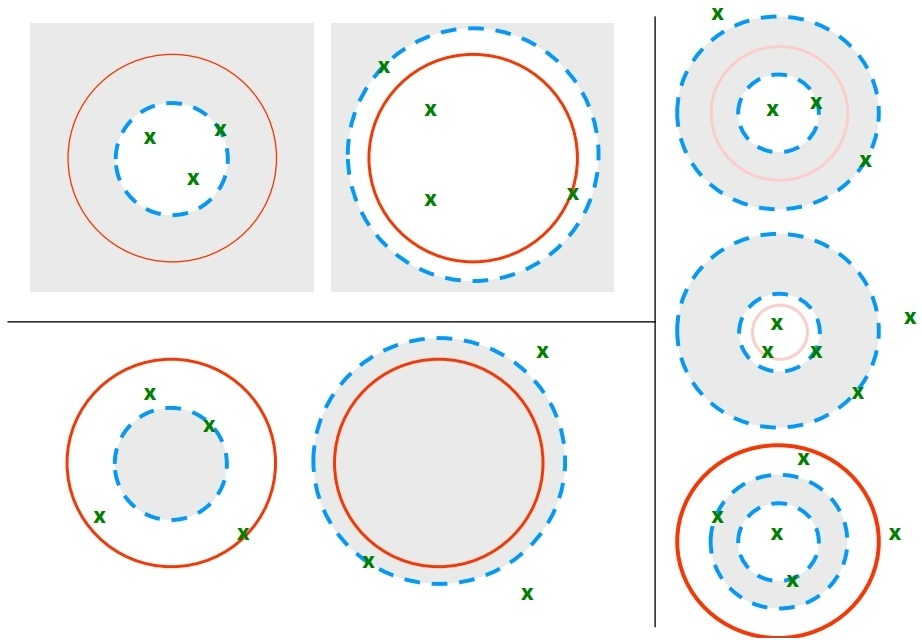
\includegraphics[width=0.6\textwidth]{chap4/img/roc_pole.png}
        \caption{ROC 与极点的关系}
        \label{fig:roc_pole}
    \end{figure}
\end{remark}

\begin{note}
    求 ROC 所求得的是级数收敛的\bd{充分条件而非必要条件},
    即,实际上 ROC 可能比所求得的更大。
\end{note}

\subsubsection{常见序列及其 ZT}

\begin{example}[单位冲激序列的 ZT]
    单位冲击序列 $\delta(n)$ 的 Z 变换为
    \begin{align*}
        \mathcal{Z}[\delta(n)] = 1, \quad (\text{ROC}: 0 \le \abs{z} \le +\infty).
    \end{align*}
    这是因为
    \begin{align*}
        \mathcal{Z}[\delta(n)] = \sum_{n=-\infty}^{+\infty} \delta(n) z^{-n} = \delta(0) = 1.
    \end{align*}
\end{example}

\begin{example}[单位阶跃序列的 ZT]
    单位阶跃序列 $u(n)$ 的 Z 变换为
    \begin{align*}
        \mathcal{Z}[u(n)] = \frac{1}{1 - z^{-1}}, \quad (\text{ROC}: \abs{z} > 1).
    \end{align*}
    这是因为
    \begin{align*}
        \mathcal{Z}[u(n)] = \sum_{n=0}^{+\infty} z^{-n} = \frac{1}{1 - z^{-1}}.
    \end{align*}
\end{example}

\begin{example}[矩形脉冲序列的 ZT]
    矩形脉冲序列 $G_N(n) = \begin{cases}
        1, & 0 \le n < N, \\
        0, & n < 0 \text{ 或 } n \ge N
    \end{cases}$ 的 Z 变换为
    \begin{align*}
        \mathcal{Z}[G_N(n)] = \frac{1 - z^{-N}}{1 - z^{-1}}, \quad (\text{ROC}: 0 < \abs{z} \le +\infty).
    \end{align*}
    这是因为
    \begin{align*}
        \mathcal{Z}[G_N(n)] = \sum_{n=0}^{N-1} z^{-n} = \frac{1 - z^{-N}}{1 - z^{-1}}.
    \end{align*}
\end{example}

\begin{example}[单位指数序列的 ZT]
    单位指数序列 $a^n u(n)$ 的 Z 变换为
    \begin{align*}
        \mathcal{Z}[a^n u(n)] = \frac{1}{1 - az^{-1}}, \quad (\text{ROC}: \abs{z} > \abs{a}).
    \end{align*}
    这是因为
    \begin{align*}
        \mathcal{Z}[a^n u(n)] = \sum_{n=0}^{+\infty} a^n z^{-n} = \frac{1}{1 - az^{-1}}.
    \end{align*}
    而 $-a^n u(-n-1)$ 的 Z 变换为
    \begin{align*}
        \mathcal{Z}[-a^n u(-n-1)] = \begin{cases}
            1/(1 - az^{-1}), & (\text{ROC}: \abs{z} < \abs{a}), \\
            0, & (\text{ROC}: \abs{z} = 0).
        \end{cases}
    \end{align*}
    这是因为
    \begin{align*}
        \mathcal{Z}[-a^n u(-n-1)] = \sum_{n=-\infty}^{-1} a^n z^{-n}
        = \begin{cases}
            1/(1 - az^{-1}), & \abs{z} < \abs{a}, \\
            0, & \abs{z} = 0.
        \end{cases}.
    \end{align*}
\end{example}

\subsubsection{ZT 的性质}

\begin{property}[ZT 是线性的]
    设 $x_1(n)$ 和 $x_2(n)$ 的 Z 变换分别为 $X_1(z)$ 和 $X_2(z)$,
    则有
    \begin{align*}
        \mathcal{Z}[a_1 x_1(n) + a_2 x_2(n)] = a_1 X_1(z) + a_2 X_2(z).
    \end{align*}
    更一般地,对于任意序列集合 $\{x_k(n)\}$ 和系数集合 $\{a_k\}$,有
    \begin{align*}
        \mathcal{Z}\left[\sum_k a_k x_k(n)\right] = \sum_k a_k \mathcal{Z}[x_k(n)] = \sum_k a_k X_k(z).
    \end{align*}
\end{property}

\begin{property}[ZT 的时域频移性质]
    设 $x(n)$ 的 Z 变换为 $X(z)$,则对于任意整数 $m$,有
    \begin{align*}
        \mathcal{Z}[x(n - m)] = z^{-m} X(z).
    \end{align*}
\end{property}

\begin{property}[ZT 的时域扩展性质]
    定义序列 $x(n)$ 以周期 $a \quad (a \in \set{Z}, a \neq 0)$ 进行时域扩展而得的序列为
    \begin{align*}
        x_{(a)}(n) = \begin{cases}
            x(n/a), & n/a \in \set{Z}, \\
            0, & n/a \notin \set{Z}.
        \end{cases}
    \end{align*}
    则有
    \begin{align*}
        \mathcal{Z}[x_{(a)}(n)] = \sum_{n=-\infty}^{+\infty} x_{(a)}(n) z^{-n} = \sum_{k=-\infty}^{+\infty} x(k) z^{-ak} = X(z^a). \quad (\text{ROC}: R_1 < \abs{z^a} < R_2).
    \end{align*}
    这里的 $a$ 称为\bd{扩展因子}。$a > 1$ 相当于在原序列每两点之间
    插入 $a - 1$ 个 $0$。$a < - 1$ 相当于原序列先反褶,再在每两点之间
    插入 $-a - 1$ 个 $0$。
\end{property}

\begin{property}[ZT 的奇偶对称性质]
    设 $x(n)$ 的 Z 变换为 $X(z)$。
    \begin{itemize}
        \item 若 $x(n)$ 是偶对称的,则
            \begin{align*}
                X(z) = \mathcal{Z}[x(n)] = \mathcal{Z}[x(-n)] = X(1/z).
            \end{align*}
        \item 若 $x(n)$ 是奇对称的,则
            \begin{align*}
                X(z) = \mathcal{Z}[x(n)] = -\mathcal{Z}[x(-n)] = -X(1/z).
            \end{align*}
    \end{itemize}
\end{property}

\begin{corollary}
    由 ZT 的奇偶对称性可以得知,如果一个偶对称或奇对称序列的 ZT 含有
    一个非零的零点(或极点)$z_0$,那么它一定含有一个相对应的零点(或极点)$1/z_0$。
\end{corollary}

\begin{property}[ZT 的时域共轭性质]
    设 $x(n)$ 的 Z 变换为 $X(z)$,则
    \begin{align*}
        \mathcal{Z}[x^*(n)] = X^*(z^*). \quad (\text{ROC}: R_1 < \abs{z} < R_2).
    \end{align*}
\end{property}

\begin{corollary}
    由 ZT 的时域共轭性可以得知,若 $x(n)$ 是实序列,则
    \begin{align*}
        X(z) = \mathcal{Z}[x(n)] = \mathcal{Z}[x^*(n)] = X^*(z^*).
    \end{align*}
    也就是说,如果一个实序列的 ZT 含有一个零点(或极点)$z_0$,
    那么它一定含有一个相对应的零点(或极点)$z_0^*$。
\end{corollary}

\begin{property}[Z 域尺度变换]
    设 $x(n)$ 的 Z 变换为 $X(z)$,则
    \begin{align*}
        \mathcal{Z}[a^nx(n)] = X(z/a), \quad (\text{ROC}: R_1 < \abs{z/a} < R_2), \\
        \mathcal{Z}[a^{-n}x(n)] = X(az), \quad (\text{ROC}: R_1 < \abs{az} < R_2), \\
        \mathcal{Z}[(-1)^nx(n)] = X(-z), \quad (\text{ROC}: R_1 < \abs{z} < R_2), \\
        \mathcal{Z}[\mathe^{\mathi\omega_0 n}x(n)] = X(z\mathe^{-\mathi\omega_0}), \quad (\text{ROC}: R_1 < \abs{z} < R_2).
    \end{align*}
    这说明可以用复指数序列来调制序列的相位特性。
\end{property}

\begin{property}[Z 域的微分性质]
    设 $x(n)$ 的 Z 变换为 $X(z)$,则
    \begin{align*}
        \mathcal{Z}[nx(n)] = -z\frac{\D}{\D{z}}X(z), \quad (\text{ROC}: R_1 < \abs{z} < R_2).
    \end{align*}
    此时 ROC 唯一可能的变换是加上或者去掉 $z = 0$ 或 $z = +\infty$。
    更进一步地,有
    \begin{align*}
        \mathcal{Z}[n^mx(n)] = \left(-z\frac{\D}{\D{z}}\right)^m X(z), \quad (\text{ROC}: R_1 < \abs{z} < R_2),
    \end{align*}
    其中 $m$ 为非负整数。
\end{property}

\begin{property}[ZT 的初值定理]
    设 $x(n)$ 的 Z 变换为 $X(z)$,则
    \begin{align*}
        x(0) = \lim_{z \to +\infty} X(z).
    \end{align*}
\end{property}

\begin{property}[ZT 的终值定理]
    设 $x(n)$ 的 Z 变换为 $X(z)$,则
    \begin{align*}
        \lim_{n \to +\infty} x(n) = \lim_{z \to 1} (z - 1)X(z).
    \end{align*}
\end{property}

\begin{remark}
    初值定理和终值定理是 Z 变换的两个重要性质。但使用条件非常苛刻,
    只有在极限存在的情况下才能使用。
    此时,$X(z)$ 的极点必须在单位圆内(如果位于单位圆上,则只能位于 $z = 1$,
    且必须是一阶极点)。
\end{remark}

\begin{property}[ZT 的时域卷积定理]
    设 $x(n)$ 和 $y(n)$ 的 Z 变换分别为 $X(z)$ 和 $Y(z)$,则
    \begin{align*}
        \mathcal{Z}[x(n) * y(n)] = X(z)Y(z).
    \end{align*}
    卷积的 ZT 的 ROC 至少是两个序列的 ROC 的交集。
    当出现\bd{零极点相抵}的情况时,ROC 可能会扩大。
\end{property}

\begin{property}[ZT 的帕斯瓦尔定理]
    设 $x(n)$ 和 $y(n)$ 的 Z 变换分别为 $X(z)$ 和 $Y(z)$,则
    \begin{align*}
        \sum_{n=-\infty}^{+\infty} x(n)y^*(n) = \frac{1}{2\pi\mathi}\oint_C X(z)Y^*(1/z^*)z^{-1} \D{z},
    \end{align*}
    其中 $C$ 为包围 ROC 的逆时针方向的简单闭合曲线。
\end{property}

\subsubsection{逆 Z 变换的求解}


\begin{exercise}
    已知某系统的差分方程如下式:
    \begin{align*}
        y(n) = x(n) - 2x(n - 2) + 0.5x(n - 4) + 0.25y(n - 2).
    \end{align*}
    \begin{enumerate}[label=(\arabic*)]
        \item 判断该系统是 IIR 型还是 FIR 型,并给出判断依据。
        \item 求该系统的传递函数 $H(z)$。
        \item 画出该系统的信号流图,分别给出直接 I 型和直接 II 型的实现。
        \item 求该系统对应的因果序列及其收敛域,并判断该状态下系统是否稳定。
    \end{enumerate}
\end{exercise}
\subsection{数字滤波器的设计}

数字滤波器的设计分为两种,一种是\bd{有限脉冲响应}(FIR)滤波器的设计,
另一种是\bd{无限脉冲响应}(IIR)滤波器的设计。

\subsubsection{低通 FIR 滤波器的设计}

由于单位冲激响应被截短成了有限项,所以滤波器的频率响应特性会发生改变。
根据经验,在设计滤波器时, 理想低通滤波器的截止频率不使用通带边缘频率,
而是使用\bd{过渡带中点的频率}。即如图 \ref{fig:low_pass_filter_fir} 所示,
\begin{align*}
    f_c = \text{设计指标要求的通道边缘频率} + \frac{\text{过渡带宽度}}{2},
\end{align*}
其中 $f_c$ 是理想低通滤波器的截止频率。

\begin{figure}[H]
    \centering
    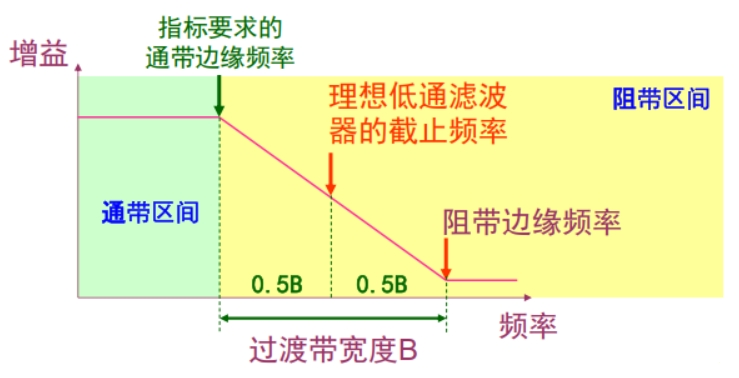
\includegraphics[width=0.8\textwidth]{chap4/img/low_pass_filter_fir.png}
    \caption{低通 FIR 滤波器设计}
    \label{fig:low_pass_filter_fir}
\end{figure}

\begin{example}[设计低通 FIR 滤波器的步骤]
    设计低通 FIR 滤波器的步骤如下:
    \begin{enumerate}
        \item 在过渡带宽度中间,选择理想低通滤波器的截止频率
            \begin{align*}
                f_c = \text{设计指标要求的通道边缘频率} + \frac{\text{过渡带宽度}}{2}.
            \end{align*}
        \item 计算截止频率的数字角频率
            \begin{align*}
                \omega_c = 2\pi \times \frac{f_c}{f_s},
            \end{align*}
            并代入
            \begin{align*}
                h(n) = \frac{\sin(\omega_c n)}{\pi n}.
            \end{align*}
        \item 从表中选择满足阻带衰减及其他要求的窗函数,计算窗内非零项的数目 $N$,
            选取满足条件的奇数 $N$,并计算窗函数 $w(n)$。
        \item 将 $w(n)$ 和 $h(n)$ 相乘,计算有限长脉冲响应 $h'(n) = w(n)h(n)$。
        \item 将脉冲右移 $\frac{N - 1}{2}$ 个单位,得到 $h''(n)$。
    \end{enumerate}
\end{example}

\begin{example}
    根据下列指标设计低通 FIR 滤波器,写出其单位冲激响应函数 $h(n)$。
    \begin{figure}[H]
        \centering
        \begin{tabular}{|c|c|}
            \hline
            通带边缘频率:$10\;\mathrm{kHz}$ & 阻带边缘频率:$22\;\mathrm{kHz}$ \\
            \hline
            采样频率:$50\;\mathrm{kHz}$ & 阻带衰减:$75\;\mathrm{dB}$ \\
            \hline
        \end{tabular}
    \end{figure}
    供设计 FIR 滤波器时参考的各种窗函数性能如下图所示(若多种同时满足,则选序号最小的):
    \begin{figure}[H]
        \centering
        \begin{tabular}{|c|c|p{5cm}|p{4cm}|c|c|}
            \hline
            \textbf{序号} & \textbf{窗类型} & \textbf{窗函数}\newline $(\abs{n} \le (N - 1) / 2)$ & \textbf{窗内项数}\newline(\text{T.W.} 是过渡带宽度) & \textbf{阻带衰减} & \textbf{通带边缘增益} \\
            \hline
            1 & 矩形 & $1$ & $0.91 f_s / \text{T.W.}$ & $21$ & $-0.9$ \\
            \hline
            2 & 汉宁 & $0.5 + 0.5\cos(2\pi n / (N-1))$ & $3.32 f_s / \text{T.W.}$ & $44$ & $-0.06$ \\
            \hline
            3 & 哈明 & $0.54 + 0.46\cos(2\pi n / (N-1))$ & $3.44 f_s / \text{T.W.}$ & $55$ & $-0.02$ \\
            \hline
            4 & 布莱克曼 & $0.42 + 0.5\cos(2\pi n / (N-1)) + 0.08\cos(4\pi n / (N-1))$ & $5.98 f_s / \text{T.W.}$ & $75$ & $-0.0014$ \\
            \hline
        \end{tabular}
    \end{figure}
\end{example}

\begin{solution}
    过渡带宽度
    \begin{align*}
        \text{T.W.} = 22 - 10 = 12\;\mathrm{kHz},
    \end{align*}
    理想低通滤波器的截止频率
    \begin{align*}
        f_c = 10 + \frac{1}{2} \times 12 = 16\;\mathrm{kHz},
    \end{align*}
    则相应的数字角频率
    \begin{align*}
        \omega_c = 2\pi \times \frac{f_c}{f_s} = 2\pi \times \frac{16}{50} = \frac{16\pi}{25}.
    \end{align*}
    计算得
    \begin{align*}
        h(n) = \frac{\sin(\omega_c n)}{\pi n} = \frac{\sin(16\pi n / 25)}{\pi n}.
    \end{align*}
    由阻带衰减为 $75\;\mathrm{dB}$ 知,应当选择布莱克曼窗。由于
    \begin{align*}
        N \ge 5.98 \times \frac{f_s}{\text{T.W.}} = 5.98 \times \frac{50}{12} \approx 24.9,
    \end{align*}
    故取 $N = 25$。则
    \begin{align*}
        w(n) = 0.42 + 0.5\cos\frac{2\pi n}{N - 1} + 0.08\cos\frac{4\pi n}{N - 1} = 0.42 + 0.5\cos\frac{\pi n}{12} + 0.08\cos\frac{\pi n}{6}.
    \end{align*}
    因此,低通 FIR 滤波器的冲激响应函数为
    \begin{align*}
        h'(n) = h(n) w(n) = \frac{\sin(16\pi n / 25)}{\pi n} \left(0.42 + 0.5\cos\frac{\pi n}{12} + 0.08\cos\frac{\pi n}{6}\right) \quad (\abs{n} \le 12).
    \end{align*}
    将其右移 $(N - 1) / 2 = 12$ 个单位,即得
    \begin{align*}
        h''(n) = \frac{\sin(16\pi (n - 12) / 25)}{\pi (n - 12)} \left(0.42 + 0.5\cos\frac{\pi (n - 12)}{12} + 0.08\cos\frac{\pi (n - 12)}{6}\right) \quad (0 \le n \le 24).
    \end{align*}
\end{solution}

\begin{exercise}
    根据下列指标设计低通 FIR 滤波器,写出其单位冲激响应函数 $h(n)$。
    \begin{figure}[H]
        \centering
        \begin{tabular}{|c|c|}
            \hline
            通带边缘频率:$2\;\mathrm{kHz}$ & 阻带边缘频率:$3\;\mathrm{kHz}$ \\
            \hline
            采样频率:$10\;\mathrm{kHz}$ & 阻带衰减:$40\;\mathrm{dB}$ \\
            \hline
        \end{tabular}
    \end{figure}
    供设计 FIR 滤波器时参考的各种窗函数性能如下图所示(若多种同时满足,则选序号最小的):
    \begin{figure}[H]
        \centering
        \begin{tabular}{|c|c|p{5cm}|p{4cm}|c|c|}
            \hline
            \textbf{序号} & \textbf{窗类型} & \textbf{窗函数}\newline $(\abs{n} \le (N - 1) / 2)$ & \textbf{窗内项数}\newline(\text{T.W.} 是过渡带宽度) & \textbf{阻带衰减} & \textbf{通带边缘增益} \\
            \hline
            1 & 矩形 & $1$ & $0.91 f_s / \text{T.W.}$ & $21$ & $-0.9$ \\
            \hline
            2 & 汉宁 & $0.5 + 0.5\cos(2\pi n / (N-1))$ & $3.32 f_s / \text{T.W.}$ & $44$ & $-0.06$ \\
            \hline
            3 & 哈明 & $0.54 + 0.46\cos(2\pi n / (N-1))$ & $3.44 f_s / \text{T.W.}$ & $55$ & $-0.02$ \\
            \hline
            4 & 布莱克曼 & $0.42 + 0.5\cos(2\pi n / (N-1)) + 0.08\cos(4\pi n / (N-1))$ & $5.98 f_s / \text{T.W.}$ & $75$ & $-0.0014$ \\
            \hline
        \end{tabular}
    \end{figure}
\end{exercise}

\begin{solution}
    过渡带宽度
    \begin{align*}
        \text{T.W.} = 3 - 2 = 1\;\mathrm{kHz},
    \end{align*}
    理想低通滤波器的截止频率
    \begin{align*}
        f_c = 2 + \frac{1}{2} \times 2 = 2.5\;\mathrm{kHz},
    \end{align*}
    则相应的数字角频率
    \begin{align*}
        \omega_c = 2\pi \times \frac{f_c}{f_s} = 2\pi \times \frac{2.5}{10} = \frac{\pi}{2}.
    \end{align*}
    计算得
    \begin{align*}
        h(n) = \frac{\sin(\omega_c n)}{\pi n} = \frac{\sin(\pi n / 2)}{\pi n}.
    \end{align*}
    由阻带衰减为 $40\;\mathrm{dB}$ 知,应当选择汉宁窗。由于
    \begin{align*}
        N \ge 3.32 \times \frac{f_s}{\text{T.W.}} = 3.32 \times \frac{10}{1} = 33.2,
    \end{align*}
    故取 $N = 35$。则
    \begin{align*}
        w(n) = 0.5 + 0.5\cos\frac{2\pi n}{N - 1} = 0.5 + 0.5\cos\frac{\pi n}{17}.
    \end{align*}
    因此,低通 FIR 滤波器的冲激响应函数为
    \begin{align*}
        h'(n) = h(n) w(n) = \frac{\sin(\pi n / 2)}{\pi n} \left(0.5 + 0.5\cos\frac{\pi n}{17}\right) \quad (\abs{n} \le 17).
    \end{align*}
    将其右移 $(N - 1) / 2 = 17$ 个单位,即得
    \begin{align*}
        h''(n) = \frac{\sin(\pi (n - 17) / 2)}{\pi (n - 17)} \left(0.5 + 0.5\cos\frac{\pi (n - 17)}{17}\right) \quad (0 \le n \le 34).
    \end{align*}
\end{solution}

\begin{exercise}
    根据下列指标设计低通 FIR 滤波器,写出其单位冲激响应函数 $h(n)$。
    \begin{figure}[H]
        \centering
        \begin{tabular}{|c|c|}
            \hline
            通带边缘频率:$3.3\;\mathrm{kHz}$ & 过渡带宽度:$4.4\;\mathrm{kHz}$ \\
            \hline
            采样频率:$22\;\mathrm{kHz}$ & 阻带衰减:$43\;\mathrm{dB}$ \\
            \hline
        \end{tabular}
    \end{figure}
    供设计 FIR 滤波器时参考的各种窗函数性能如下图所示(若多种同时满足,则选序号最小的):
    \begin{figure}[H]
        \centering
        \begin{tabular}{|c|c|p{5cm}|p{4cm}|c|c|}
            \hline
            \textbf{序号} & \textbf{窗类型} & \textbf{窗函数}\newline $(\abs{n} \le (N - 1) / 2)$ & \textbf{窗内项数}\newline(\text{T.W.} 是过渡带宽度) & \textbf{阻带衰减} & \textbf{通带边缘增益} \\
            \hline
            1 & 矩形 & $1$ & $0.91 f_s / \text{T.W.}$ & $21$ & $-0.9$ \\
            \hline
            2 & 汉宁 & $0.5 + 0.5\cos(2\pi n / (N-1))$ & $3.32 f_s / \text{T.W.}$ & $44$ & $-0.06$ \\
            \hline
            3 & 哈明 & $0.54 + 0.46\cos(2\pi n / (N-1))$ & $3.44 f_s / \text{T.W.}$ & $55$ & $-0.02$ \\
            \hline
            4 & 布莱克曼 & $0.42 + 0.5\cos(2\pi n / (N-1)) + 0.08\cos(4\pi n / (N-1))$ & $5.98 f_s / \text{T.W.}$ & $75$ & $-0.0014$ \\
            \hline
        \end{tabular}
    \end{figure}
\end{exercise}

\begin{solution}
    截止频率
    \begin{align*}
        f_c = 3.3 + \frac{1}{2} \times 4.4 = 5.5\;\mathrm{kHz},
    \end{align*}
    则
    \begin{align*}
        \omega_c = 2\pi \times \frac{f_c}{f_s} = 2\pi \times \frac{5.5}{22} = \frac{\pi}{2}.
    \end{align*}
    计算得
    \begin{align*}
        h(n) = \frac{\sin(\omega_c n)}{\pi n} = \frac{\sin(\pi n / 2)}{\pi n}.
    \end{align*}
    由阻带衰减为 $43\;\mathrm{dB}$ 知,应当选择汉宁窗。由于
    \begin{align*}
        N \ge 3.32 \times \frac{f_s}{\text{T.W.}} = 3.32 \times \frac{22}{4.4} = 16.6,
    \end{align*}
    故取 $N = 17$。则
    \begin{align*}
        w(n) = 0.5 + 0.5\cos\frac{2\pi n}{N - 1} = 0.5 + 0.5\cos\frac{\pi n}{8}.
    \end{align*}
    因此,低通 FIR 滤波器的冲激响应函数为
    \begin{align*}
        h'(n) = h(n) w(n) = \frac{\sin(\pi n / 2)}{\pi n} \left(0.5 + 0.5\cos\frac{\pi n}{8}\right) \quad (\abs{n} \le 8).
    \end{align*}
    将其右移 $(N - 1) / 2 = 8$ 个单位,即得
    \begin{align*}
        h''(n) = \frac{\sin(\pi (n - 8) / 2)}{\pi (n - 8)} \left(0.5 + 0.5\cos\frac{\pi (n - 8)}{8}\right) \quad (0 \le n \le 16).
    \end{align*}
\end{solution}

\subsubsection{带通 FIR 滤波器的设计}

频率响应函数需要在频域移动到新的位置,频移的方法:将脉冲响应与余弦函数相乘:
\begin{align*}
    h'(n) = h(n)w(n)\cos(\omega_0 n),
\end{align*}
其中 $w(n)$ 是窗函数,$\omega_0$ 是带通滤波器的中心频率,如图 \ref{fig:band_pass_filter_fir} 所示。

\begin{figure}[H]
    \centering
    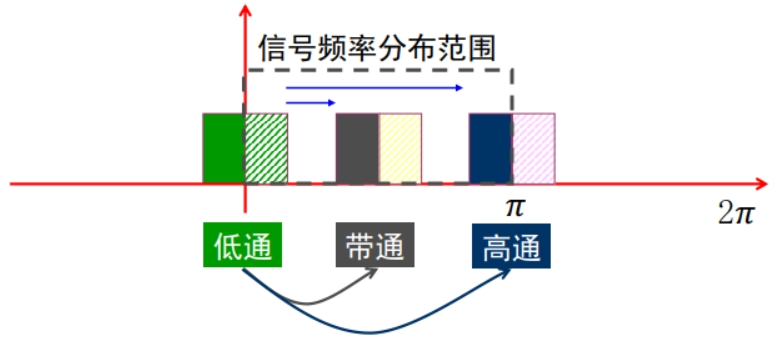
\includegraphics[width=0.8\textwidth]{chap4/img/band_pass_filter_fir.png}
    \caption{带通 FIR 滤波器设计}
    \label{fig:band_pass_filter_fir}
\end{figure}

\begin{exercise}
    根据下列指标设计带通 FIR 滤波器,写出其单位冲激响应函数 $h(n)$。
    \begin{figure}[H]
        \centering
        \begin{tabular}{|c|c|}
            \hline
            带通中心频率:$4\;\mathrm{kHz}$ & 过渡带宽度:$0.5\;\mathrm{kHz}$ \\
            \hline
            通带边缘频率:$3.5\;\mathrm{kHz}, 4.5\;\mathrm{kHz}$ & 阻带衰减:$50\;\mathrm{dB}$ \\
            \hline
            采样频率:$22\;\mathrm{kHz}$ & \\
            \hline
        \end{tabular}
    \end{figure}
    供设计 FIR 滤波器时参考的各种窗函数性能如下图所示(若多种同时满足,则选序号最小的):
    \begin{figure}[H]
        \centering
        \begin{tabular}{|c|c|p{5cm}|p{4cm}|c|c|}
            \hline
            \textbf{序号} & \textbf{窗类型} & \textbf{窗函数}\newline $(\abs{n} \le (N - 1) / 2)$ & \textbf{窗内项数}\newline(\text{T.W.} 是过渡带宽度) & \textbf{阻带衰减} & \textbf{通带边缘增益} \\
            \hline
            1 & 矩形 & $1$ & $0.91 f_s / \text{T.W.}$ & $21$ & $-0.9$ \\
            \hline
            2 & 汉宁 & $0.5 + 0.5\cos(2\pi n / (N-1))$ & $3.32 f_s / \text{T.W.}$ & $44$ & $-0.06$ \\
            \hline
            3 & 哈明 & $0.54 + 0.46\cos(2\pi n / (N-1))$ & $3.44 f_s / \text{T.W.}$ & $55$ & $-0.02$ \\
            \hline
            4 & 布莱克曼 & $0.42 + 0.5\cos(2\pi n / (N-1)) + 0.08\cos(4\pi n / (N-1))$ & $5.98 f_s / \text{T.W.}$ & $75$ & $-0.0014$ \\
            \hline
        \end{tabular}
    \end{figure}
\end{exercise}

\begin{solution}
    首先考虑其对应的低通 FIR 滤波器,截止频率
    \begin{align*}
        f_c = 4.5 - 4 + \frac{1}{2} \times 0.5 = 0.75\;\mathrm{kHz},
    \end{align*}
    则
    \begin{align*}
        \omega_c = 2\pi \times \frac{f_c}{f_s} = 2\pi \times \frac{0.75}{22} = \frac{3\pi}{44}.
    \end{align*}
    计算得
    \begin{align*}
        h(n) = \frac{\sin(\omega_c n)}{\pi n} = \frac{\sin(3\pi n / 44)}{\pi n}.
    \end{align*}
    由阻带衰减为 $50\;\mathrm{dB}$ 知,应当选择哈明窗。由于
    \begin{align*}
        N \ge 3.44 \times \frac{f_s}{\text{T.W.}} = 3.44 \times \frac{22}{0.5} = 151.36,
    \end{align*}
    故取 $N = 153$。则
    \begin{align*}
        w(n) = 0.54 + 0.46\cos\frac{2\pi n}{N - 1} = 0.54 + 0.46\cos\frac{\pi n}{76}.
    \end{align*}
    带通中心频率为 $f_0 = 4\;\mathrm{kHz}$,对应的数字角频率为
    \begin{align*}
        \omega_0 = 2\pi \times \frac{f_0}{f_s} = 2\pi \times \frac{4}{22} = \frac{4\pi}{11}.
    \end{align*}
    因此,带通 FIR 滤波器的冲激响应函数为
    \begin{align*}
        h'(n) = h(n) w(n) \cos(\omega_0 n) = \frac{\sin(3\pi n / 44)}{\pi n} \left(0.54 + 0.46\cos\frac{\pi n}{76}\right) \cos\frac{4\pi n}{11} \quad (\abs{n} \le 76).
    \end{align*}
    将其右移 $(N - 1) / 2 = 76$ 个单位,即得
    \begin{align*}
        h''(n) = \frac{\sin(3\pi (n - 76) / 44)}{\pi (n - 76)} \left(0.54 + 0.46\cos\frac{\pi (n - 76)}{76}\right) \cos\frac{4\pi (n - 76)}{11} \quad (0 \le n \le 152).
    \end{align*}
\end{solution}

\begin{exercise}
    在以 $22\;\mathrm{kHz}$ 采集的某种信号数据中,夹杂了许多低频和高频的干扰信号。
    请你选择一种满足条件的窗函数,设计一个带通 FIR 滤波器去除这些干扰信号。
    要求设计的带通滤波器的带通中心频率为 $5\;\mathrm{kHz}$,
    通带边缘频率为 $4\;\mathrm{kHz}$ 和 $6\;\mathrm{kHz}$,过渡带宽度为 $1\;\mathrm{kHz}$,
    且至少满足阻带衰减 $45\;\mathrm{dB}$。请写出一种符合设计要求的滤波器的
    单位冲激响应函数 $h(n)$。
    供设计 FIR 滤波器时参考的各种窗函数性能如下图所示(若多种同时满足,则选序号最小的):
    \begin{figure}[H]
        \centering
        \begin{tabular}{|c|c|p{5cm}|p{4cm}|c|c|}
            \hline
            \textbf{序号} & \textbf{窗类型} & \textbf{窗函数}\newline $(\abs{n} \le (N - 1) / 2)$ & \textbf{窗内项数}\newline(\text{T.W.} 是过渡带宽度) & \textbf{阻带衰减} & \textbf{通带边缘增益} \\
            \hline
            1 & 矩形 & $1$ & $0.91 f_s / \text{T.W.}$ & $21$ & $-0.9$ \\
            \hline
            2 & 汉宁 & $0.5 + 0.5\cos(2\pi n / (N-1))$ & $3.32 f_s / \text{T.W.}$ & $44$ & $-0.06$ \\
            \hline
            3 & 哈明 & $0.54 + 0.46\cos(2\pi n / (N-1))$ & $3.44 f_s / \text{T.W.}$ & $55$ & $-0.02$ \\
            \hline
            4 & 布莱克曼 & $0.42 + 0.5\cos(2\pi n / (N-1)) + 0.08\cos(4\pi n / (N-1))$ & $5.98 f_s / \text{T.W.}$ & $75$ & $-0.0014$ \\
            \hline
        \end{tabular}
    \end{figure}
\end{exercise}

\begin{solution}
    首先考虑其对应的低通 FIR 滤波器,截止频率
    \begin{align*}
        f_c = 5 - 4 + \frac{1}{2} \times 1 = 1.5\;\mathrm{kHz},
    \end{align*}
    则
    \begin{align*}
        \omega_c = 2\pi \times \frac{f_c}{f_s} = 2\pi \times \frac{1.5}{22} = \frac{3\pi}{22}.
    \end{align*}
    计算得
    \begin{align*}
        h(n) = \frac{\sin(\omega_c n)}{\pi n} = \frac{\sin(3\pi n / 22)}{\pi n}.
    \end{align*}
    由阻带衰减为 $45\;\mathrm{dB}$ 知,应当选择哈明窗。由于
    \begin{align*}
        N \ge 3.44 \times \frac{f_s}{\text{T.W.}} = 3.44 \times \frac{22}{1} = 75.68,
    \end{align*}
    故取 $N = 77$。则
    \begin{align*}
        w(n) = 0.54 + 0.46\cos\frac{2\pi n}{N - 1} = 0.54 + 0.46\cos\frac{\pi n}{38}.
    \end{align*}
    带通中心频率为 $f_0 = 5\;\mathrm{kHz}$,对应的数字角频率为
    \begin{align*}
        \omega_0 = 2\pi \times \frac{f_0}{f_s} = 2\pi \times \frac{5}{22} = \frac{5\pi}{11}.
    \end{align*}
    因此,带通 FIR 滤波器的冲激响应函数为
    \begin{align*}
        h'(n) = h(n) w(n) \cos(\omega_0 n) = \frac{\sin(3\pi n / 22)}{\pi n} \left(0.54 + 0.46\cos\frac{\pi n}{38}\right) \cos\frac{5\pi n}{11} \quad (\abs{n} \le 38).
    \end{align*}
    将其右移 $(N - 1) / 2 = 38$ 个单位,即得
    \begin{align*}
        h''(n) = \frac{\sin(3\pi (n - 38) / 22)}{\pi (n - 38)} \left(0.54 + 0.46\cos\frac{\pi (n - 38)}{38}\right) \cos\frac{5\pi (n - 38)}{11} \quad (0 \le n \le 76).
    \end{align*}
\end{solution}

\begin{note}
    带通滤波器还可以使用一个高通滤波器和一个低通滤波器级联实现。如图 \ref{fig:band_pass_filter_cascade} 所示。
    \begin{figure}[H]
        \centering
        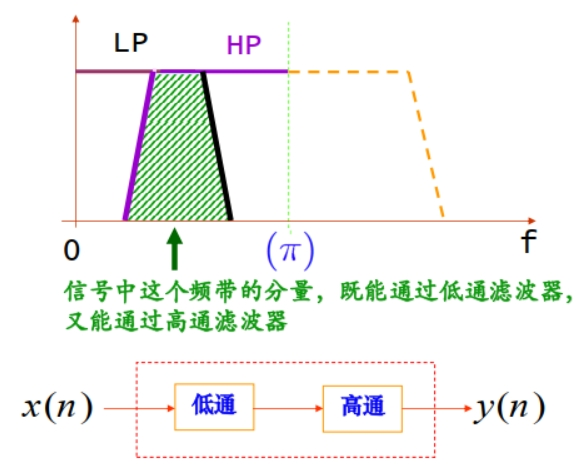
\includegraphics[width=0.6\textwidth]{chap4/img/band_pass_filter_cascade.png}
        \caption{带通滤波器级联}
        \label{fig:band_pass_filter_cascade}
    \end{figure}
    因此,
    \begin{align*}
        H_{\text{BP}}(\omega) & = H_{\text{LP}}(\omega) \cdot H_{\text{HP}}(\omega), \\
        h_{\text{BP}}(n) & = h_{\text{LP}}(n) * h_{\text{HP}}(n).
    \end{align*}
\end{note}

\subsubsection{高通 FIR 滤波器的设计}

高通 FIR 滤波器的设计与低通 FIR 滤波器的设计类似,只是将带通滤波器的中心频率移动到高频区域,
此时 $\omega_0 = \pi$。

\begin{exercise}
    根据下列指标设计高通 FIR 滤波器,写出其单位冲激响应函数 $h(n)$。
    \begin{figure}[H]
        \centering
        \begin{tabular}{|c|c|}
            \hline
            通带边缘频率:$8\;\mathrm{kHz}$ & 阻带边缘频率:$6\;\mathrm{kHz}$ \\
            \hline
            采样频率:$22\;\mathrm{kHz}$ & 阻带衰减:$40\;\mathrm{dB}$ \\
            \hline
        \end{tabular}
    \end{figure}
    供设计 FIR 滤波器时参考的各种窗函数性能如下图所示(若多种同时满足,则选序号最小的):
    \begin{figure}[H]
        \centering
        \begin{tabular}{|c|c|p{5cm}|p{4cm}|c|c|}
            \hline
            \textbf{序号} & \textbf{窗类型} & \textbf{窗函数}\newline $(\abs{n} \le (N - 1) / 2)$ & \textbf{窗内项数}\newline(\text{T.W.} 是过渡带宽度) & \textbf{阻带衰减} & \textbf{通带边缘增益} \\
            \hline
            1 & 矩形 & $1$ & $0.91 f_s / \text{T.W.}$ & $21$ & $-0.9$ \\
            \hline
            2 & 汉宁 & $0.5 + 0.5\cos(2\pi n / (N-1))$ & $3.32 f_s / \text{T.W.}$ & $44$ & $-0.06$ \\
            \hline
            3 & 哈明 & $0.54 + 0.46\cos(2\pi n / (N-1))$ & $3.44 f_s / \text{T.W.}$ & $55$ & $-0.02$ \\
            \hline
            4 & 布莱克曼 & $0.42 + 0.5\cos(2\pi n / (N-1)) + 0.08\cos(4\pi n / (N-1))$ & $5.98 f_s / \text{T.W.}$ & $75$ & $-0.0014$ \\
            \hline
        \end{tabular}
    \end{figure}
\end{exercise}

\begin{solution}
    首先考虑其对应的低通 FIR 滤波器,截止频率
    \begin{align*}
        f_c = \frac{22}{2} - 8 + \frac{1}{2} \times (8 - 6) = 4\;\mathrm{kHz},
    \end{align*}
    则
    \begin{align*}
        \omega_c = 2\pi \times \frac{f_c}{f_s} = 2\pi \times \frac{4}{22} = \frac{4\pi}{11}.
    \end{align*}
    计算得
    \begin{align*}
        h(n) = \frac{\sin(\omega_c n)}{\pi n} = \frac{\sin(4\pi n / 11)}{\pi n}.
    \end{align*}
    由阻带衰减为 $40\;\mathrm{dB}$ 知,应当选择汉宁窗。由于
    \begin{align*}
        N \ge 3.32 \times \frac{f_s}{\text{T.W.}} = 3.32 \times \frac{22}{8 - 6} = 36.52,
    \end{align*}
    故取 $N = 37$。则
    \begin{align*}
        w(n) = 0.5 + 0.5\cos\frac{2\pi n}{N - 1} = 0.5 + 0.5\cos\frac{\pi n}{18}.
    \end{align*}
    因此,高通 FIR 滤波器的冲激响应函数为
    \begin{align*}
        h'(n) = h(n) w(n) \cos(\pi n) = \frac{\sin(4\pi n / 11)}{\pi n} \left(0.5 + 0.5\cos\frac{\pi n}{18}\right) \cos(\pi n) \quad (\abs{n} \le 18).
    \end{align*}
    将其右移 $(N - 1) / 2 = 18$ 个单位,即得
    \begin{align*}
        h''(n) = \frac{\sin(4\pi (n - 18) / 11)}{\pi (n - 18)} \left(0.5 + 0.5\cos\frac{\pi (n - 18)}{18}\right) \cos(\pi (n - 18)) \quad (0 \le n \le 36).
    \end{align*}
\end{solution}

\begin{exercise}
    在以 $22\;\mathrm{kHz}$ 采集某种信号数据的过程中,虽然满足采样定理,但因受到环境的影响,
    采集的数据中夹杂了许多低频干扰信号。请选择一种满足条件的窗函数(若多种同时满足,
    则选序号较小的),设计一个高通 FIR 滤波器去除这些干扰信号。
    要求设计的高通滤波器的通带边缘频率为 $8\;\mathrm{kHz}$,
    过渡带宽度为 $2\;\mathrm{kHz}$,且至少满足阻带衰减 $45\;\mathrm{dB}$。
    请写出一种符合设计要求的滤波器的单位冲激响应函数 $h(n)$。
    \begin{figure}[H]
        \centering
        \begin{tabular}{|c|c|p{5cm}|p{4cm}|c|c|}
            \hline
            \textbf{序号} & \textbf{窗类型} & \textbf{窗函数}\newline $(\abs{n} \le (N - 1) / 2)$ & \textbf{窗内项数}\newline(\text{T.W.} 是过渡带宽度) & \textbf{阻带衰减} & \textbf{通带边缘增益} \\
            \hline
            1 & 矩形 & $1$ & $0.91 f_s / \text{T.W.}$ & $21$ & $-0.9$ \\
            \hline
            2 & 汉宁 & $0.5 + 0.5\cos(2\pi n / (N-1))$ & $3.32 f_s / \text{T.W.}$ & $44$ & $-0.06$ \\
            \hline
            3 & 哈明 & $0.54 + 0.46\cos(2\pi n / (N-1))$ & $3.44 f_s / \text{T.W.}$ & $55$ & $-0.02$ \\
            \hline
            4 & 布莱克曼 & $0.42 + 0.5\cos(2\pi n / (N-1)) + 0.08\cos(4\pi n / (N-1))$ & $5.98 f_s / \text{T.W.}$ & $75$ & $-0.0014$ \\
            \hline
        \end{tabular}
    \end{figure}
\end{exercise}

\begin{solution}
    首先考虑其对应的低通 FIR 滤波器,截止频率
    \begin{align*}
        f_c = \frac{22}{2} - 8 + \frac{1}{2} \times 2 = 4\;\mathrm{kHz},
    \end{align*}
    则
    \begin{align*}
        \omega_c = 2\pi \times \frac{f_c}{f_s} = 2\pi \times \frac{4}{22} = \frac{4\pi}{11}.
    \end{align*}
    计算得
    \begin{align*}
        h(n) = \frac{\sin(\omega_c n)}{\pi n} = \frac{\sin(4\pi n / 11)}{\pi n}.
    \end{align*}
    由阻带衰减为 $45\;\mathrm{dB}$ 知,应当选择哈明窗。由于
    \begin{align*}
        N \ge 3.44 \times \frac{f_s}{\text{T.W.}} = 3.44 \times \frac{22}{2} = 37.84,
    \end{align*}
    故取 $N = 39$。则
    \begin{align*}
        w(n) = 0.54 + 0.46\cos\frac{2\pi n}{N - 1} = 0.54 + 0.46\cos\frac{\pi n}{19}.
    \end{align*}
    因此,高通 FIR 滤波器的冲激响应函数为
    \begin{align*}
        h'(n) = h(n) w(n) \cos(\pi n) = \frac{\sin(4\pi n / 11)}{\pi n} \left(0.54 + 0.46\cos\frac{\pi n}{19}\right) \cos(\pi n) \quad (\abs{n} \le 19).
    \end{align*}
    将其右移 $(N - 1) / 2 = 19$ 个单位,即得
    \begin{align*}
        h''(n) = \frac{\sin(4\pi (n - 19) / 11)}{\pi (n - 19)} \left(0.54 + 0.46\cos\frac{\pi (n - 19)}{19}\right) \cos(\pi (n - 19)) \quad (0 \le n \le 38).
    \end{align*}
\end{solution}

\begin{exercise}
    根据下列指标设计高通 FIR 滤波器,写出其单位冲激响应函数 $h(n)$。
    \begin{figure}[H]
        \centering
        \begin{tabular}{|c|c|}
            \hline
            通带边缘频率:$8.8\;\mathrm{kHz}$ & 过渡带宽度:$4.4\;\mathrm{kHz}$ \\
            \hline
            采样频率:$22\;\mathrm{kHz}$ & 阻带衰减:$35\;\mathrm{dB}$ \\
            \hline
        \end{tabular}
    \end{figure}
    供设计 FIR 滤波器时参考的各种窗函数性能如下图所示(若多种同时满足,则选序号最小的):
    \begin{figure}[H]
        \centering
        \begin{tabular}{|c|c|p{5cm}|p{4cm}|c|c|}
            \hline
            \textbf{序号} & \textbf{窗类型} & \textbf{窗函数}\newline $(\abs{n} \le (N - 1) / 2)$ & \textbf{窗内项数}\newline(\text{T.W.} 是过渡带宽度) & \textbf{阻带衰减} & \textbf{通带边缘增益} \\
            \hline
            1 & 矩形 & $1$ & $0.91 f_s / \text{T.W.}$ & $21$ & $-0.9$ \\
            \hline
            2 & 汉宁 & $0.5 + 0.5\cos(2\pi n / (N-1))$ & $3.32 f_s / \text{T.W.}$ & $44$ & $-0.06$ \\
            \hline
            3 & 哈明 & $0.54 + 0.46\cos(2\pi n / (N-1))$ & $3.44 f_s / \text{T.W.}$ & $55$ & $-0.02$ \\
            \hline
            4 & 布莱克曼 & $0.42 + 0.5\cos(2\pi n / (N-1)) + 0.08\cos(4\pi n / (N-1))$ & $5.98 f_s / \text{T.W.}$ & $75$ & $-0.0014$ \\
            \hline
        \end{tabular}
    \end{figure}
\end{exercise}

\begin{solution}
    首先考虑其对应的低通 FIR 滤波器,截止频率
    \begin{align*}
        f_c = \frac{22}{2} - 8.8 + \frac{1}{2} \times 4.4 = 4.4\;\mathrm{kHz},
    \end{align*}
    则
    \begin{align*}
        \omega_c = 2\pi \times \frac{f_c}{f_s} = 2\pi \times \frac{4.4}{22} = \frac{2\pi}{5}.
    \end{align*}
    计算得
    \begin{align*}
        h(n) = \frac{\sin(\omega_c n)}{\pi n} = \frac{\sin(2\pi n / 5)}{\pi n}.
    \end{align*}
    由阻带衰减为 $35\;\mathrm{dB}$ 知,应当选择汉宁窗。由于
    \begin{align*}
        N \ge 3.32 \times \frac{f_s}{\text{T.W.}} = 3.32 \times \frac{22}{4.4} = 16.6,
    \end{align*}
    故取 $N = 17$。则
    \begin{align*}
        w(n) = 0.5 + 0.5\cos\frac{2\pi n}{N - 1} = 0.5 + 0.5\cos\frac{\pi n}{8}.
    \end{align*}
    因此,高通 FIR 滤波器的冲激响应函数为
    \begin{align*}
        h'(n) = h(n) w(n) \cos(\pi n) = \frac{\sin(2\pi n / 5)}{\pi n} \left(0.5 + 0.5\cos\frac{\pi n}{8}\right) \cos(\pi n) \quad (\abs{n} \le 8).
    \end{align*}
    将其右移 $(N - 1) / 2 = 8$ 个单位,即得
    \begin{align*}
        h''(n) = \frac{\sin(2\pi (n - 8) / 5)}{\pi (n - 8)} \left(0.5 + 0.5\cos\frac{\pi (n - 8)}{8}\right) \cos(\pi (n - 8)) \quad (0 \le n \le 16).
    \end{align*}
\end{solution}

\subsubsection{带阻 FIR 滤波器的设计}

带阻滤波器可以通过一个低通滤波器和一个高通滤波器并联实现。如图 \ref{fig:band_stop_filter_parallel} 所示。
\begin{figure}[H]
    \centering
    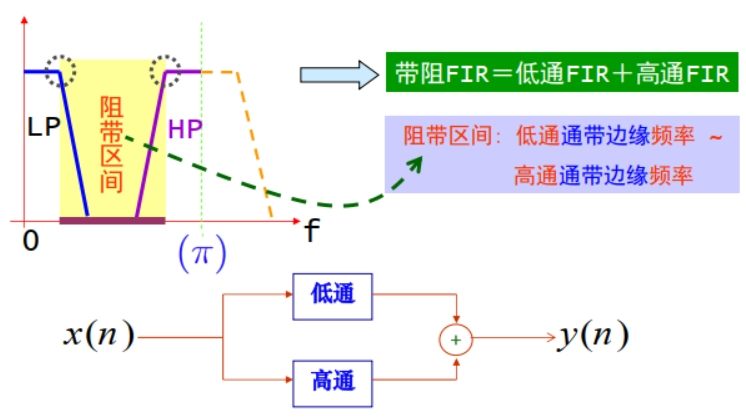
\includegraphics[width=0.6\textwidth]{chap4/img/band_stop_filter_parallel.png}
    \caption{带阻滤波器并联}
    \label{fig:band_stop_filter_parallel}
\end{figure}
因此,
\begin{align*}
    H_{\text{BS}}(\omega) & = H_{\text{LP}}(\omega) + H_{\text{HP}}(\omega), \\
    h_{\text{BS}}(n) & = h_{\text{LP}}(n) + h_{\text{HP}}(n).
\end{align*}

